% !TeX root = ../main.tex
% !TeX root = ../main.tex
% Add the above to each chapter to make compiling the PDF easier in some editors.

\chapter{Fundamentals of TUMLive}\label{chapter:fundamentals}

\section{GoCast Lecture Streaming Service}

\subsection{Overview}

GoCast is a fully self-hosted platform for live-streaming and recording of lectures, in use at the \ac{TUM} as TUM-Live.
TUM-Live offers live and on-demand videos of lectures and events from the department of informatics and mathematics at \ac{TUM}. 
It's main features include:

\begin{itemize}
    \item Fully automatic Live-Streaming from Auditoriums based on lecture schedules as imported from CAMPUSonline.
    \item Self-service interface for lecturers to schedule and manage their videos.
    \item Automated import of lectures and enrollment of students from CAMPUSonline.
    \item Self-streaming via OBS, Zoom, etc.
    \item Automatic recording of live-streams.
    \item Video on demand uploads.
    \item Automatic post-processing of recordings.
    \begin{itemize}
        \item Detects silence in videos and makes them skip-able.
        \item Transcribes videos and makes them searchable.
        \item Generates Thumbnails.
    \end{itemize}
    \item Live Chat for listeners to ask questions.
    \begin{itemize}
        \item Polls can be created by lecturers.
        \item Questions can be upvoted by listeners.
        \item Questions can be marked as answered or hidden.
    \end{itemize}
\end{itemize}

\subsection{Current System Architecture}

At the core of the GoCast system, there is the main \ac{API} built on the GoGin Framework and connected to a MariaDB Database. Its main functionality is to manage users, courses, streams, synchronize events between TUM-Live and CAMPUSonline. For user authentication, it uses the provided services of \ac{TUM}'s \ac{LDAP} and \ac{SAML} to allow users to authenticate themselves with their university credentials using \ac{SSO}. 
Next, whenever a lecture is recorded or livestreamed, the video data is processed by a TUM-Live Worker which then transcodes and segments the video into MPEG-2 compressed video transport stream files. These segments are then uploaded to a shared storage using the VOD Service component so that they can then later be distributed by the Edge Server.

\begin{figure}[htpb]
    \centering
    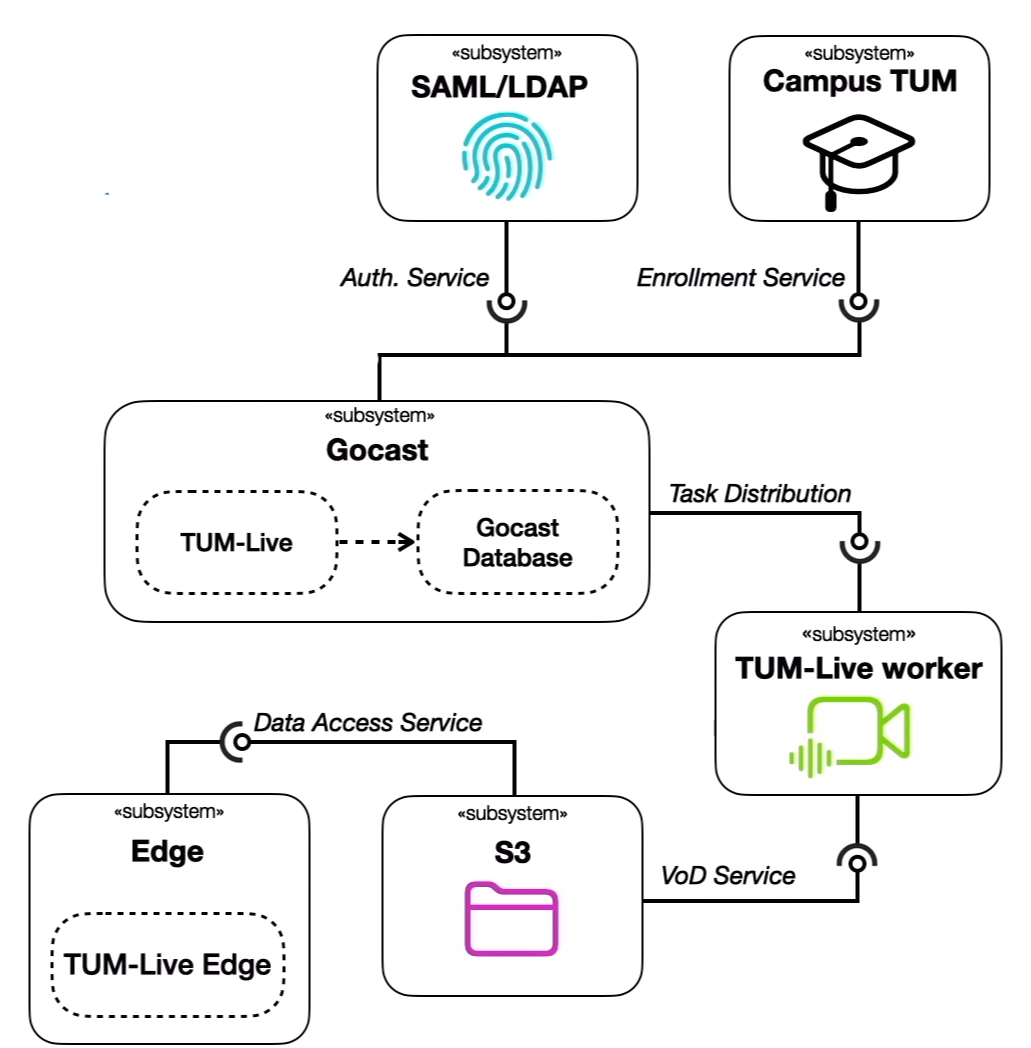
\includegraphics[width=320pt]{images/OldDeploymentDiagram.png}
    \caption[Subsystem Decomposition]{Subsystem Decomposition Model of TUM-Live}\label{fig:system-architecture}
\end{figure}

\subsection{Stats and Metrics of TUM-Live}

Since its creation in February of 2021, GoCast has been used to stream thousands of hours of video every semester for more than 150 courses and 15.000 Students. The source code is open-source, accessible at \href{https://github.com/TUM-Dev/gocast}{github.com/TUM-Dev/gocast} and licensed under the MIT license.

